\label{chap:users_manual}

TODO: screenshots

\section{Registration and Login}

We require the users to be logged in to the application during their work. We do so to enable the users to save their work a return to it another time. 

\subsection{Registration and Basic Login}

First option how to get an account to the application is to register and get a user name and password. Anyway, if you have a Google or Seznam account we recommend you to use the second way of registration, via those two services.

\begin{figure}
\begin{center}
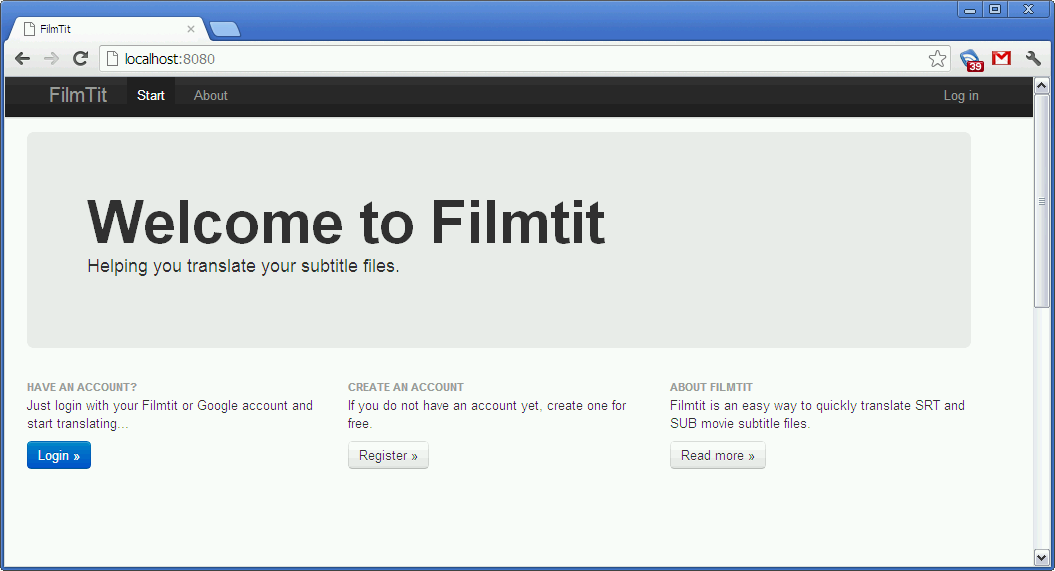
\includegraphics[scale=0.4]{figures/user_manual/welcome_screen.png}
\end{center}
\caption{Welcome screen of the application.}
\label{fig:welcome}
\end{figure}

After opening the welcome screen click on the welcome screen (figure \ref{fig:welcome}) or clicking on login button and selecting the first tab in opened dialog (figure \ref{fig:register_login}).

After that you are requested to choose a user name, fill in a valid a email address and type twice the password you would like to use. Because the application does not contain any sensitive information we try to keep the registration and login process as simple as possible and there are no requirement on the strength of the password. After the successful registration you will receive an email confirming the registration.

\begin{figure}
\begin{center}
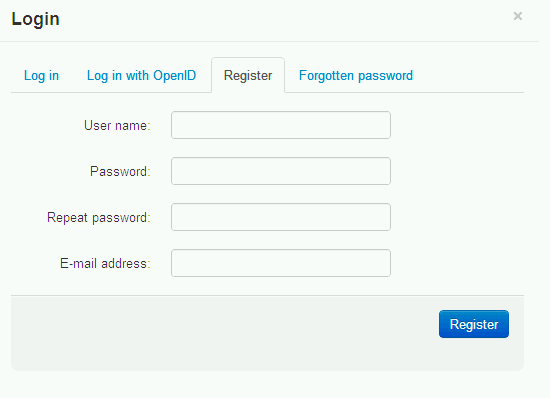
\includegraphics[scale=0.4]{figures/user_manual/register.png}~~~~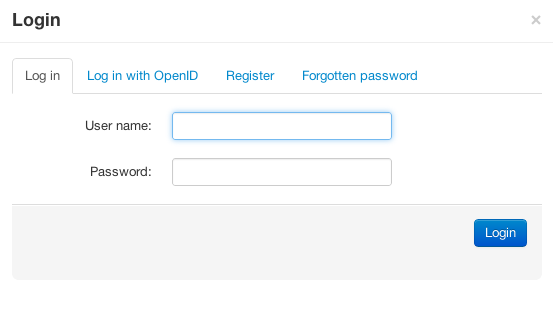
\includegraphics[scale=0.4]{figures/user_manual/login.png}
\end{center}
\caption{Registration form and login form.}
\end{figure}

You are automatically logged after the registration. For logging in next time, click on the login button on the welcome screen and fill in your user name and password (figure \ref{fig:register_login}). If you want to be logged in permanently see you change it in your settings, see section \ref{sec:settings}.

\subsection{OpenID}

Another option how to log in to the application is using Google, Yahoo or Seznam account. After choosing the service you want to use a pop-up window is opened. It may happen that your browser blocks this window. If it happens you need to allow the pop-up window to continue the logging process.

You will see the login form of the service you have chosen. If you are already logged in the service you will see just the confirmation request to allow the Filmtit application to access your account data (it is your user name, first name, surname, email and gender, depending on what you filled in in the particular service and what you allowed to be provided to the third party applications, but it is never the password to the original service). After submitting your user name and user password and confirming that the Filmit application can receive your authentication data the pop-up window will be automatically closed. Within few seconds after that you will be redirected to the list of documents you own. Is is empty at the time first you log in.

You are registered automatically on first successful login. You also automatically get a user name and password for the Basic Login, which is sent to your e-mail address upon registration (if your OpenID provider provides us with one) and can be changed in the Settings.

\subsection{Forgotten Password}

Another issue connected to login is the 

\section{Changing the User's Settings}
\label{sec:settings}

\subsection{Account and Logging in}
\subsubsection{User name}
\subsubsection{New password}

Muste retype into Repeat new password.

\subsubsection{E-mail address}
\subsubsection{Stay logged in}

\subsection{Translation Workspace}
\subsubsection{Maximum number of suggestions to show for each line}
\subsubsection{Include machine translation}

\section{Creating a New Document}

In the application we call a subtitle file as document. Creating a document means loading a subtitle file in the source language and starting translating it. You can create a new document either by clicking on the "Create a new document" button in the document list or by clicking the "New document" link in the top line.

\begin{figure}
\begin{center}
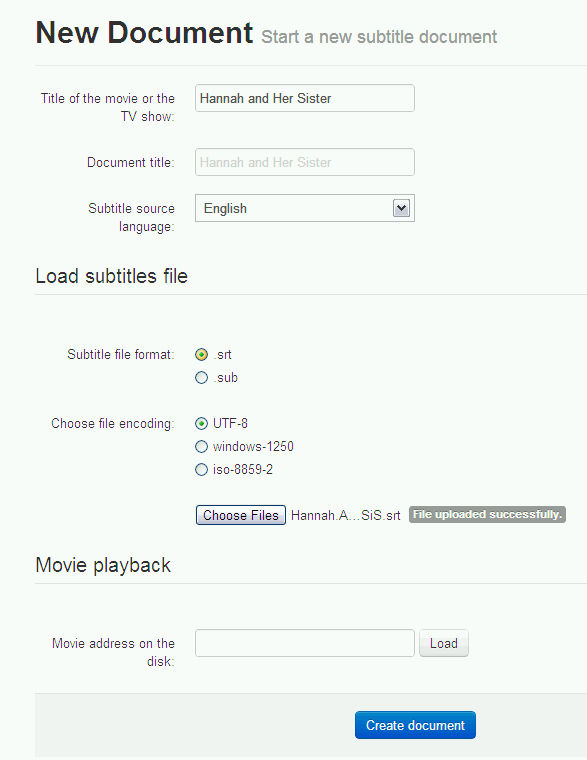
\includegraphics[scale=0.4]{figures/user_manual/new_document.png}
\end{center}
\caption{Form for creating a new document.}
\end{figure}

While creating a document you are asked to fill in the movie title and a document title in case you want to name it differently than the movie title. In the case of TV series please fill in the name of the series, not the name of the particular episode. An example of it can be to type "Lost" as the movie title and "Lost S01E01" as a document title. The you are asked to choose the source language of the subtitles, encoding of the subtitle file and the path to the actual subtitle file you would like to translate.


movie file

\section{Document Editing}

suggestions

can continue in offline mode

\section{Offline Mode}

bound to computer, browser and user

\section{Operations with Documents}

export

delete

changing title, media source